\subsection{Canal de Comunicação 3}

\begin{questions}
\question{
Considere um canal de comunicação conforme ilustrado abaixo.

   \begin{figure}[h!]
   \centering
   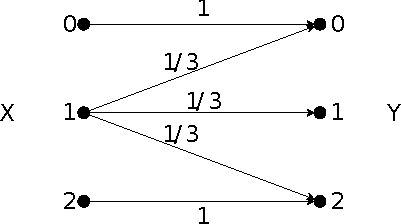
\includegraphics[width=0.3\textwidth]{../images/canalm.pdf}
   \caption{Canal de comunicação.}
   \label{fig:canal}
   \end{figure}


Para determinar a capacidade de um canal, devemos encontrar a distribuição sobre $X$
que otimiza a informação mútua entre a entrada e saída. Pela simetria do canal em questão,
e pelo fato de que a informação mútua é côncava nas probabilidades, podemos concluir
que para otimizar a transmissão de informação no canal, devemos requerer que a 
distribuição em $X$ seja tal que os símbolos $0$ e $2$ possuam a mesma probabilidade $p$.
\begin{parts}
\part 
Determine a capacidade deste canal.

\part 
Determine a distribuição em $X$ que atinge esta capacidade.
\end{parts}
(Não é necessário mostrar que a derivada segunda é negativa no ponto de distribuição encontrado.)

(Lembrete: $\log_b (x) = \log_a(x) / \log_a(b)$.)

}

\begin{solution}
O problema nos fornece que $\Pr(X=0) = \Pr(X=2) = p$ e, por conseguinte, $\Pr(X=1)=1-2p$.

A capacidade do canal é dada por:
\begin{align}
C &= \max_{p(x)} I(X;Y) = \max_{p(x)} \left( H(Y) - H(Y|X) \right) \nonumber \\
  &= \max_{p(x)} \left( H(Y) - \left( p\underbrace{H(Y|X=0)}_{=0} + (1-2p)H(Y|X=1) + p\underbrace{H(Y|X=2)}_{=0} \right) \right) \nonumber \\
  &= \max_{p(x)} \left( H(Y) - (1-2p) H\left(\frac{1}{3},\frac{1}{3},\frac{1}{3}\right) \right) = \max_{p(x)} \left( H(Y) - (1-2p) \log 3 \right) .
\end{align}
Para calcular $H(Y)$ devemos determinar a distribuição em $Y$. Podemos verificar que
teremos $\Pr(Y=0)=\Pr(Y=2)=p+\frac{1}{3}(1-2p)=\frac{1+p}{3}$ e $\Pr(Y=1)=\frac{1-2p}{3}$. Assim, poderemos
expressar $H(Y)$ da seguinte forma:
\begin{align}
H(Y) &= H\left( \frac{1+p}{3}, \frac{1-2p}{3}, \frac{1+p}{3} \right) \nonumber \\
     &= - 2 \frac{1+p}{3} \log \frac{1+p}{3} - \frac{1-2p}{3} \log \frac{1-2p}{3} .
\end{align}
Teremos assim
\begin{equation}
C = \max_{p(x)} \left( \underbrace{ - 2 \frac{1+p}{3} \log \frac{1+p}{3} - \frac{1-2p}{3} \log \frac{1-2p}{3} - (1-2p) \log 3 }_{I_p(X;Y)} \right) .
\end{equation}

Para determinar o ponto de máximo, devemos encontrar o ponto em que a derivada é igual a zero. Para tanto, iremos
primeiramente reescrever $I_p(X;Y)$ em nats:
\begin{equation}
I_p(X;Y) = \frac{-2(1+p)}{3 \ln 2} \ln \frac{1+p}{3} - \frac{1-2p}{3\ln2} \ln \frac{1-2p}{3} - \frac{(1-2p)}{\ln 2} \ln 3 \quad \text{(nats)}.
\end{equation}

E assim, a derivada será
\begin{align}
\frac{\partial }{\partial p} I_p(X;Y) &= - \frac{2}{3 \ln 2} \ln \frac{1+p}{3} - \frac{2(1+p)}{3 \ln 2} \frac{3}{1+p} 
                                                + \frac{2}{3\ln2} \ln \frac{1-2p}{3} + \frac{2(1-2p)}{3\ln2} \frac{3}{1-2p}
                                                + \frac{2}{\ln 2} \ln 3 \nonumber \\
                &= \frac{2}{3\ln2} \left( \ln \frac{1-2p}{3} - \ln \frac{1+p}{3} \right) - \frac{2}{\ln2} + \frac{2}{\ln2} + \frac{2}{\ln 2} \ln 3 \nonumber \\
                &= \frac{2}{3\ln2} \ln \frac{1-2p}{1+p} + \frac{2}{\ln2} \ln 3 \quad \text{(nats)} \nonumber \\
                &= \frac{2}{3} \log \frac{1-2p}{1+p} + 2 \log 3 \quad \text{(bits)}
\end{align}
Queremos $\frac{\partial }{\partial p} I_p(X;Y) = 0$, ou seja,
\begin{align}
\frac{2}{3} \log \frac{1-2p}{1+p} &= -  2 \log 3 \nonumber \\
\log \frac{1-2p}{1+p} &= - 3 \log 3 \nonumber \\
\frac{1-2p}{1+p} &= 2^{- 3 \log 3} \nonumber \\
\frac{1-2p}{1+p} &= \frac{1}{27} \nonumber \\
27 - 54 p &= 1 + p \nonumber \\
- 55 p &= - 26 \nonumber \\
p &=& \frac{26}{55}
\end{align}

Note que a derivada segunda de $I_p(X;Y)$ é 
\begin{align}
\frac{\partial^2 }{\partial p^2} I_p(X;Y) &=  \frac{2}{3\ln2} \frac{1+p}{1-2p} \frac{-2(1+p) - (1-2p)}{(1+p)^2} \nonumber \\
        &=  \frac{2}{3\ln2} \frac{1+p}{1-2p} \frac{-3}{(1+p)^2} \nonumber \\
        &= - \frac{2}{\ln2} \frac{1}{1-2p} \frac{1}{1+p} = \frac{2}{\ln2} \frac{1}{2p^2 + p - 1} 
\end{align}
Como $0 \leq p \leq \frac{1}{2}$, teremos a derivada segunda sempre negativa, o que era de se esperar, já que
$I_p(X;Y)$ é uma função côncava em $p$. Por conseguinte, o ponto encontrada é um ponto de máximo.

A capacidade do canal será dada por
\begin{align}
C &= H\left( \frac{1 + 26/55}{3}, \frac{1 - 2\times 26/55}{3}, \frac{1 + 26/55}{3} \right) - (1 - 2\times 26/55) \log 3 \\
  &= H\left( \frac{27}{55}, \frac{1}{55}, \frac{27}{55} \right) - \frac{3}{55} \log 3 \approx 1,0265 .
\end{align}


\end{solution}
\end{questions}
